\chapter{\acl{ser} Pipeline}
\label{chapter:ser_conf}

In this section, we present an audio pipeline for performing \ac{ser} on a video conference system. This pipeline can be used both online and offline time and includes several stages, each of which plays an essential role in properly identifying emotional content from the audio signal.

\section{Data Consumption}

The first step of the pipeline is to continuously consume the binary audio data of a video conference participant.

According to a \citeyear{Liu2022} article on pause duration of English speech \cite{Liu2022}, the mean pause duration for commas ranged from 0.51 to 0.78 seconds, while the mean pause duration for periods ranged from 1.40 to 1.43 seconds. Since we want to capture sentences/utterances, we decided to feed the pipeline with audio data corresponding to 1 second, which allows for smaller pauses such as breathing or commas during a segment and at the same time, separates sentences.

\section{Normalization}

The next step is converting the consumed binary data to an array of floats, and afterward, normalizing the audio signal. The normalization consists of, when necessary, resampling the audio to a sampling rate of 16000 Hz and converting the signal to mono by averaging samples across the channels, recurring to the Librosa toolkit \cite{Librosa}. These operations are necessary so that the audio can be accepted and interpreted by the machine learning models that will follow and analyze it.

\section{\acl{vad*}}

The third step of the pipeline is to detect voiced speech of the previously consumed second of audio, using a \ac{vad*} model.

We chose the sileroVAD tool \cite{SileroVAD}, as it is an open-source algorithm that provides accurate results in real-time. It is specifically designed for low-resource environments and can work efficiently on devices with limited processing power.

SileroVAD is based on a deep learning model trained on a large corpus of audio data. This means that it can detect voice activity even in noisy environments or when the speaker's voice is weak. This is crucial for our pipeline, since preprocessing, such as noise reduction or trimming, on unvoiced data would be a waste of resources. This allows us to only do that audio preprocessing before an audio segment is detected to be classified.

This \ac{vad*} algorithm also returns a confidence level associated with the detection of voiced speech, which allows us to fine-tune the minimum value of confidence to consider a voiced segment.

\section{Speech Segmentation}

Emotions are usually short-lived, and the speech remains invariant for a brief period. Speech segmentation is the process in which the continuous speech signals are partitioned into short-length segments while maintaining the emotional information suitable for being inputted to \ac{ser} models.

The strategy for our segmentation is to create voiced segments with a minimum of 1 second of duration and at most 8 seconds, which provides a way to detect emotions in real-time as a person speaks one or more complete sentences. The pipeline consumes 1 second of audio, it stores the segment if there is enough confidence that it detected voice activity, if it does not pass the threshold and it has previously saved any audio segment, it feeds it to a \ac{ser} model. When the saved segment reaches a maximum of 8 seconds, it also performs the classification. It is important to note that these minimum and maximum duration values can be altered to fit different situations and needs, and also, the audio preprocessing techniques (noise reduction and trimming) are executed after the pipeline generates the audio segments to be used by the \ac{ser} models.


\section{Pipeline Validation}

To validate the effectiveness of our proposed pipeline, we conducted a few tests using the \ac{iemo} session files. These files involve two speakers, one female, and one male, interacting with each other in scripted and improvised scenarios to elicit emotions.

Figure \ref{fig:iemo_pipeline} depicts an audio signal from a session that was manually annotated to label the frames with emotions for both genders and the combination of both speakers. Additionally, the figure displays the voiced segments that our pipeline detected and performed \ac{ser}.

\begin{figure}[H]
	\centering
	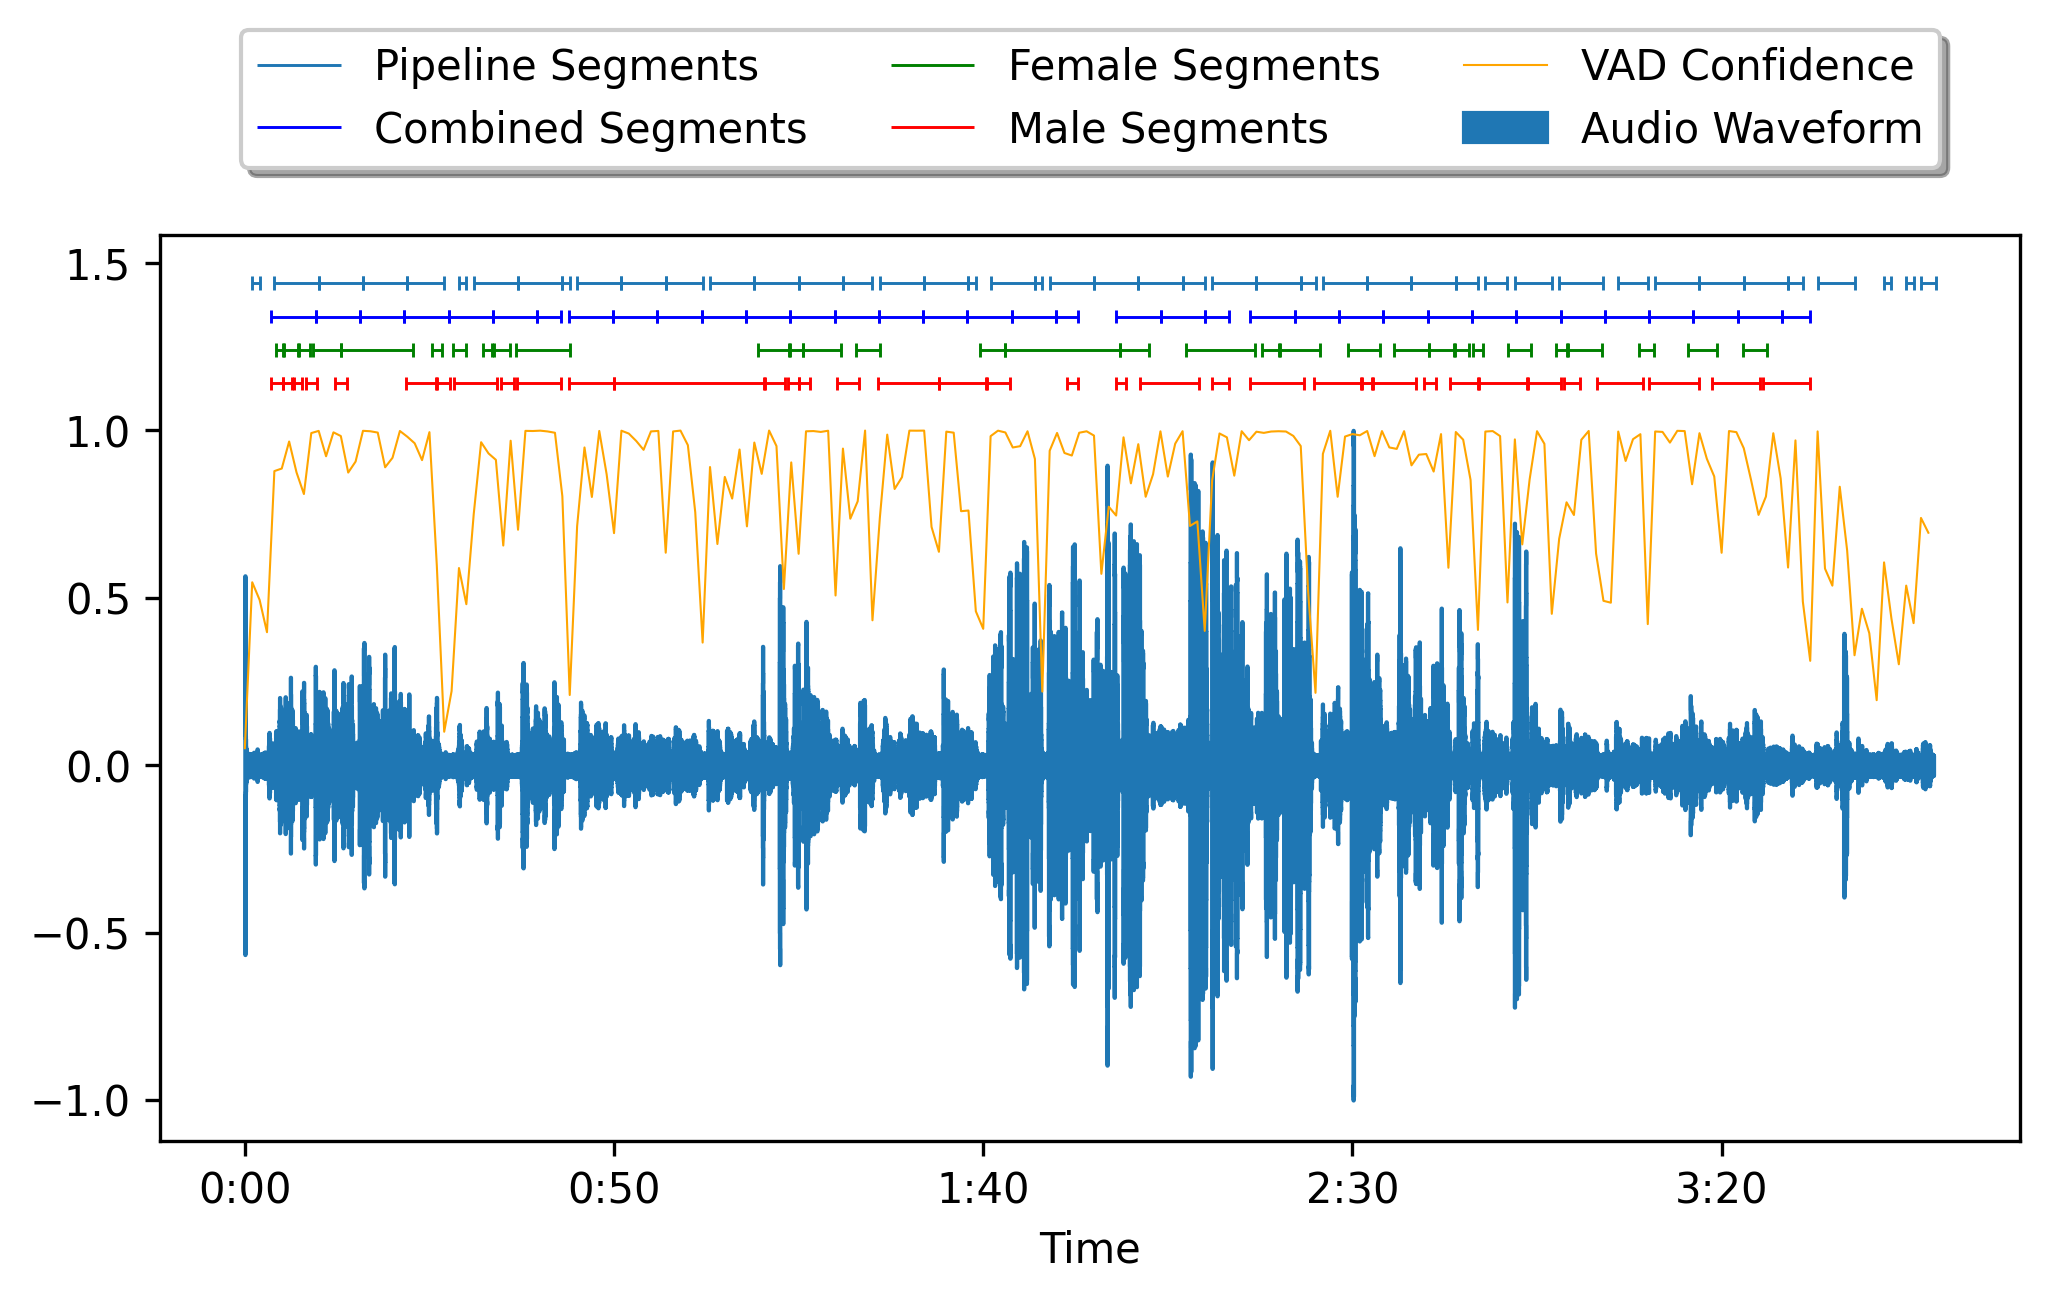
\includegraphics[width=\textwidth]{figs/6_video_conf_ser/pipeline.png}
	\caption{\ac{iemo} session annotated and detected from our developed pipeline segments.}
	\label{fig:iemo_pipeline}
\end{figure}

The efficacy of the pipeline was confirmed by its ability to detect voiced segments in the same intervals as those of the combined segments. To further test the pipeline, we passed all 11 hours of \ac{iemo} audio data through it and compared the predicted emotions with the dataset annotations. For this test, it was used an AMD Ryzen 5 5600X 6-core processor, and for classifying the detected segments, the traditional model was selected.

Table \ref{tab:iemopipeline} shows the emotions annotated in the \ac{iemo} dataset, along with the predicted emotions resulting from our pipeline.

\begin{table}[H]
	\centering
	\caption{Annotated emotions of the \ac{iemo} dataset and the pipeline's predicted segments.}
	\label{tab:iemopipeline}
	\begin{tabular}{lrr}
		\toprule
		Emotions & Dataset Labeled Segments & Pipeline Predicted Segments \\
		\midrule
		Neutral & 1708 & 1292 \\
		Happiness & 1636 & 2930 \\
		Angry & 1103 & 2144 \\
		Sadness & 1084 & 1332 \\
		Non-Identified & 2510 & - \\
		Frustration & 1849 & - \\
		Surprise	& 107 & - \\
		Fear & 40 & - \\
		Disgust & 2 & - \\
		\bottomrule
	\end{tabular}
\end{table}

\section{Discussion}

The pipeline was capable of processing the entire 11-hour audio data in just 15 minutes, including the time the model took to make predictions, which demonstrates that the pipeline is capable of detecting emotions in real-time, by continuously processing audio segments as they arrive.

In total, the dataset comprises 10,039 annotated segments, out of which the pipeline detected 7,698 segments. This is in line with our expectations, as the pipeline only considers segments with at least 1 second of audio data, and the dataset contains a lot of shorter audio. As for the distribution of predicted emotions, we anticipated that each emotion would have a similar number of predictions of the 4 emotions it was trained, given that it was trained using utterances from the same dataset.

The development of the pipeline represents a significant step forward in improving the user experience in video conference systems. With the pipeline integrated into the system, participants will have access to real-time emotional feedback. This feedback can help participants understand their emotional states, identify potential areas of conflict or misunderstanding, and make more informed decisions about how to interact with others at the conference. It is also important to note that certain configuration values may need adjustments on different use case scenarios, such as the minimum and maximum duration of the segments, the voiced speech confidence level, and also, since the classifiers can return the probabilities of each emotion, a minimum level of confidence for the segment's predicted emotion.

In conclusion, the integration of the pipeline into video conference systems, when employed with an efficient \ac{ser} classifier, has the potential to revolutionize communications in virtual environments, and, to can create more positive and productive interactions between people.
